\chapter{Opis projektnog zadatka}
		
		
		
		Tema našeg projektnog rada je izrada web aplikacije \textit{"BytePit"} koja omogućuje korisnicima sudjelovanje u programerskim natjecanjima i provjeru riješenih zadataka. Ideja je da naša stranica ima sve potrebno za obavljanje natjecanja poput registracije korisnika, uključivanje u natjecanje, pribavljanje zadataka, vrednovanje priloženih rješenja, prikaz dosadašnjih uspjeha natjecatelja i još mnogo toga.
	
		Neregistrirani korisnik može se registrirati definirajući registrira li se kao \textbf{voditelj} ili \textbf{natjecatelj}.
		Za registraciju korisnika potrebno je  unijeti \begin{packed_item}
			\item korisničko ime
			\item fotografiju
			\item lozinku
			\item ime
			\item prezime
			\item email adresu
		\end{packed_item}
		Uspješnost registracije potvrđuje se preko email adrese dok  voditelja dodatno potvrđuje i administrator.
		
		\textbf{\textit{Neregistrirani korisnik}} na web stranici može vidjeti kalendar s natjecanjima te pregledati rezultate prethodnih natjecanja - rang listu te sve zadatke koje su korisnici predali na tom natjecanju. Svi registrirani korisnici automatski nasljeđuju sve mogućnosti koje neregistrirani korisnici imaju.
		
		\textbf{\textit{Registrirani korisnik}} može vidjeti kalendar s aktualnim natjecanjima kojima može pristupiti te virtualnim natjecanjima koja može rješavati za vježbu. Prilikom sudjelovanja u natjecanju korisnik može koristiti playground pomoću kojeg provjerava točnost svog rješenja, a zatim može učitati datoteku s programskim kodom koja predstavlja konačno rješenje u aplikaciju. Također može pristupiti stranici  za vježbu na kojoj bira želi li rješavati zadatke pojedinačno ili pokrenuti opciju virtalnog natjecanja. Na stranici "korisnici" može pregledavati profile svih registriranih korisnika te uređivati svoj profil. Na stranici "rezultati" registriranom korisniku omogućuje se opcija preuzimanja svih predanih rješenja zadatka ukoliko ga je riješio u potpunosti točno. 
		
		
	    \textbf{\textit{Natjecatelj}} je registrirani korisnik koji sudjeluje u natjecanjima. Na njegovom profilu prikazana je statistika s podacima o broju predanih i točnih programskih rješenja. Prikazani su i pehari za ona natjecanja na kojima je sudjelovao i osvojio jedno od prva tri mjesta.
	    
	    \textbf{\textit{Voditelj}} je registrirani korisnik koji ima ovlasti kreiranja sadržaja. Moguće je kreirati pojedinačni zadatak ili novo natjecanje. 
	    Nakon kreiranja, novi je sadržaj moguće uređivati.
	    Na njegovom profilu vidljivi su svi javni zadatci koje je kreirao i kalendar sa svim natjecanjima koja je izradio.
	    
	    \textbf{\textit{Administrator}} nasljeđuje sve ovlasti registriranih korisnika. Dodatno mu je omogućeno uređivanje svih korisničkih profila, svih zadataka i svih budućih natjecanja (aktualna i prošla natjecanja ne mogu se više uređivati). Njegov zadatak je i potvrđivanje novoregistriranih voditelja natjecanja što može napraviti klikom na gumb na profilu novog voditelja. \\
	
		\noindent{\Large {Provedba natjecanja}}\\
		Kada dođe vrijeme koje je voditelj postavio kao početak natjecanja, zadatci ispita postaju vidljivi aktivnim natjecateljima. Za svaki zadatak natjecatelji mogu testirati točnost svog rješenja pomoću prozora za testiranje te priložiti datoteku s programskim kodom u jeziku Java. Pristupanje natjecanju omogućeno je u periodu trajanja natjecanja, a jednom kada mu se pristupi može ga se rješavati onoliko vremena koliko je vremensko ograničenje rješavanja svih zadataka. Natjecanju je moguće pristupiti samo jednom. Korisnik može pristupiti rezultatima tek kad natjecanje više nije aktivno. Rezultati se prikazuju oblikom rang liste svih sudionika poredanih silazno po prikupljenom broju bodova. Vidljiv je i popis i statistika svih rješenja koja su korisnici predali na natjecanju, po zadatcima i po korisnicima. Pri kalkulaciji broja bodova uzima se u obzir postotak točnosti i isteklo vrijeme. Onima koji su se plasirali na prva tri mjesta pridodaje se slika pehara na njihovom profilu. Po završetku natjecanja svi zadatci koji su bili privatni postaju javni i vidljivi su na stranici za vježbu, a natjecanje postaje virtualno.\\
		
		
		\noindent{\Large {Virtualno natjecanje}}\\
		Virtualno natjecanje je koncept osmišljen kako bi natjecatelji mogli provjeriti koliko su se dobro pripremili za nadolazeće natjecanje. Virtualnom natjecanju se može pristupiti preko kalendara i preko stranice za vježbu. Postoje dvije vrste virtualnog natjecanja: nasumično generirano natjecanje, u kojem aplikacija nasumično odabire pet zadataka iz baze, te simulacija prethodno održanog natjecanja koje je potrebno izabrati iz kalendara. Po završetku korisniku se prikazuje rang lista s ukupno ostvarenim brojem bodova, a ukoliko već postoji rang lista za to natjecanje prikazuje mu se i njegov virtualni rang.  \\
		
		\noindent{\Large {Slične aplikacije}}\\
		Već postojeća aplikacija vrlo slična ovoj je Edgar koji se koristi na FER-u za provođenje ispita i laboratorijskih vježbi.	S obzirom na to da je svrha te aplikacije ipak drugačija od naše, postoje neke značajne razlike. Dok se za registrirani pristup našoj aplikaciji korisnik sam prijavljuje i čeka potvrdu administratora, u Edgaru to čini administrator samostalno dodavajući korisnike (kojima se kasnije dodijele njihovi pristupni podaci). Zbog same razlike u namjeni, predana rješenja se drugačije boduju (nekim stalnim brojem bodova, bez ovisnosti o vremenu). Također, studentu prijavljenom u sustav nije omogućen pregled tuđih rješenja kao što je to slučaj u našoj aplikaciji, kao ni pristup pojedinačnim zadatcima: moguće je samo pokrenuti probni ispit ili vježbu, bez mogućnosti odabira pojedinog zadatka (slika  \ref{fig:pocstr}).\\
			\begin{figure}[H]
			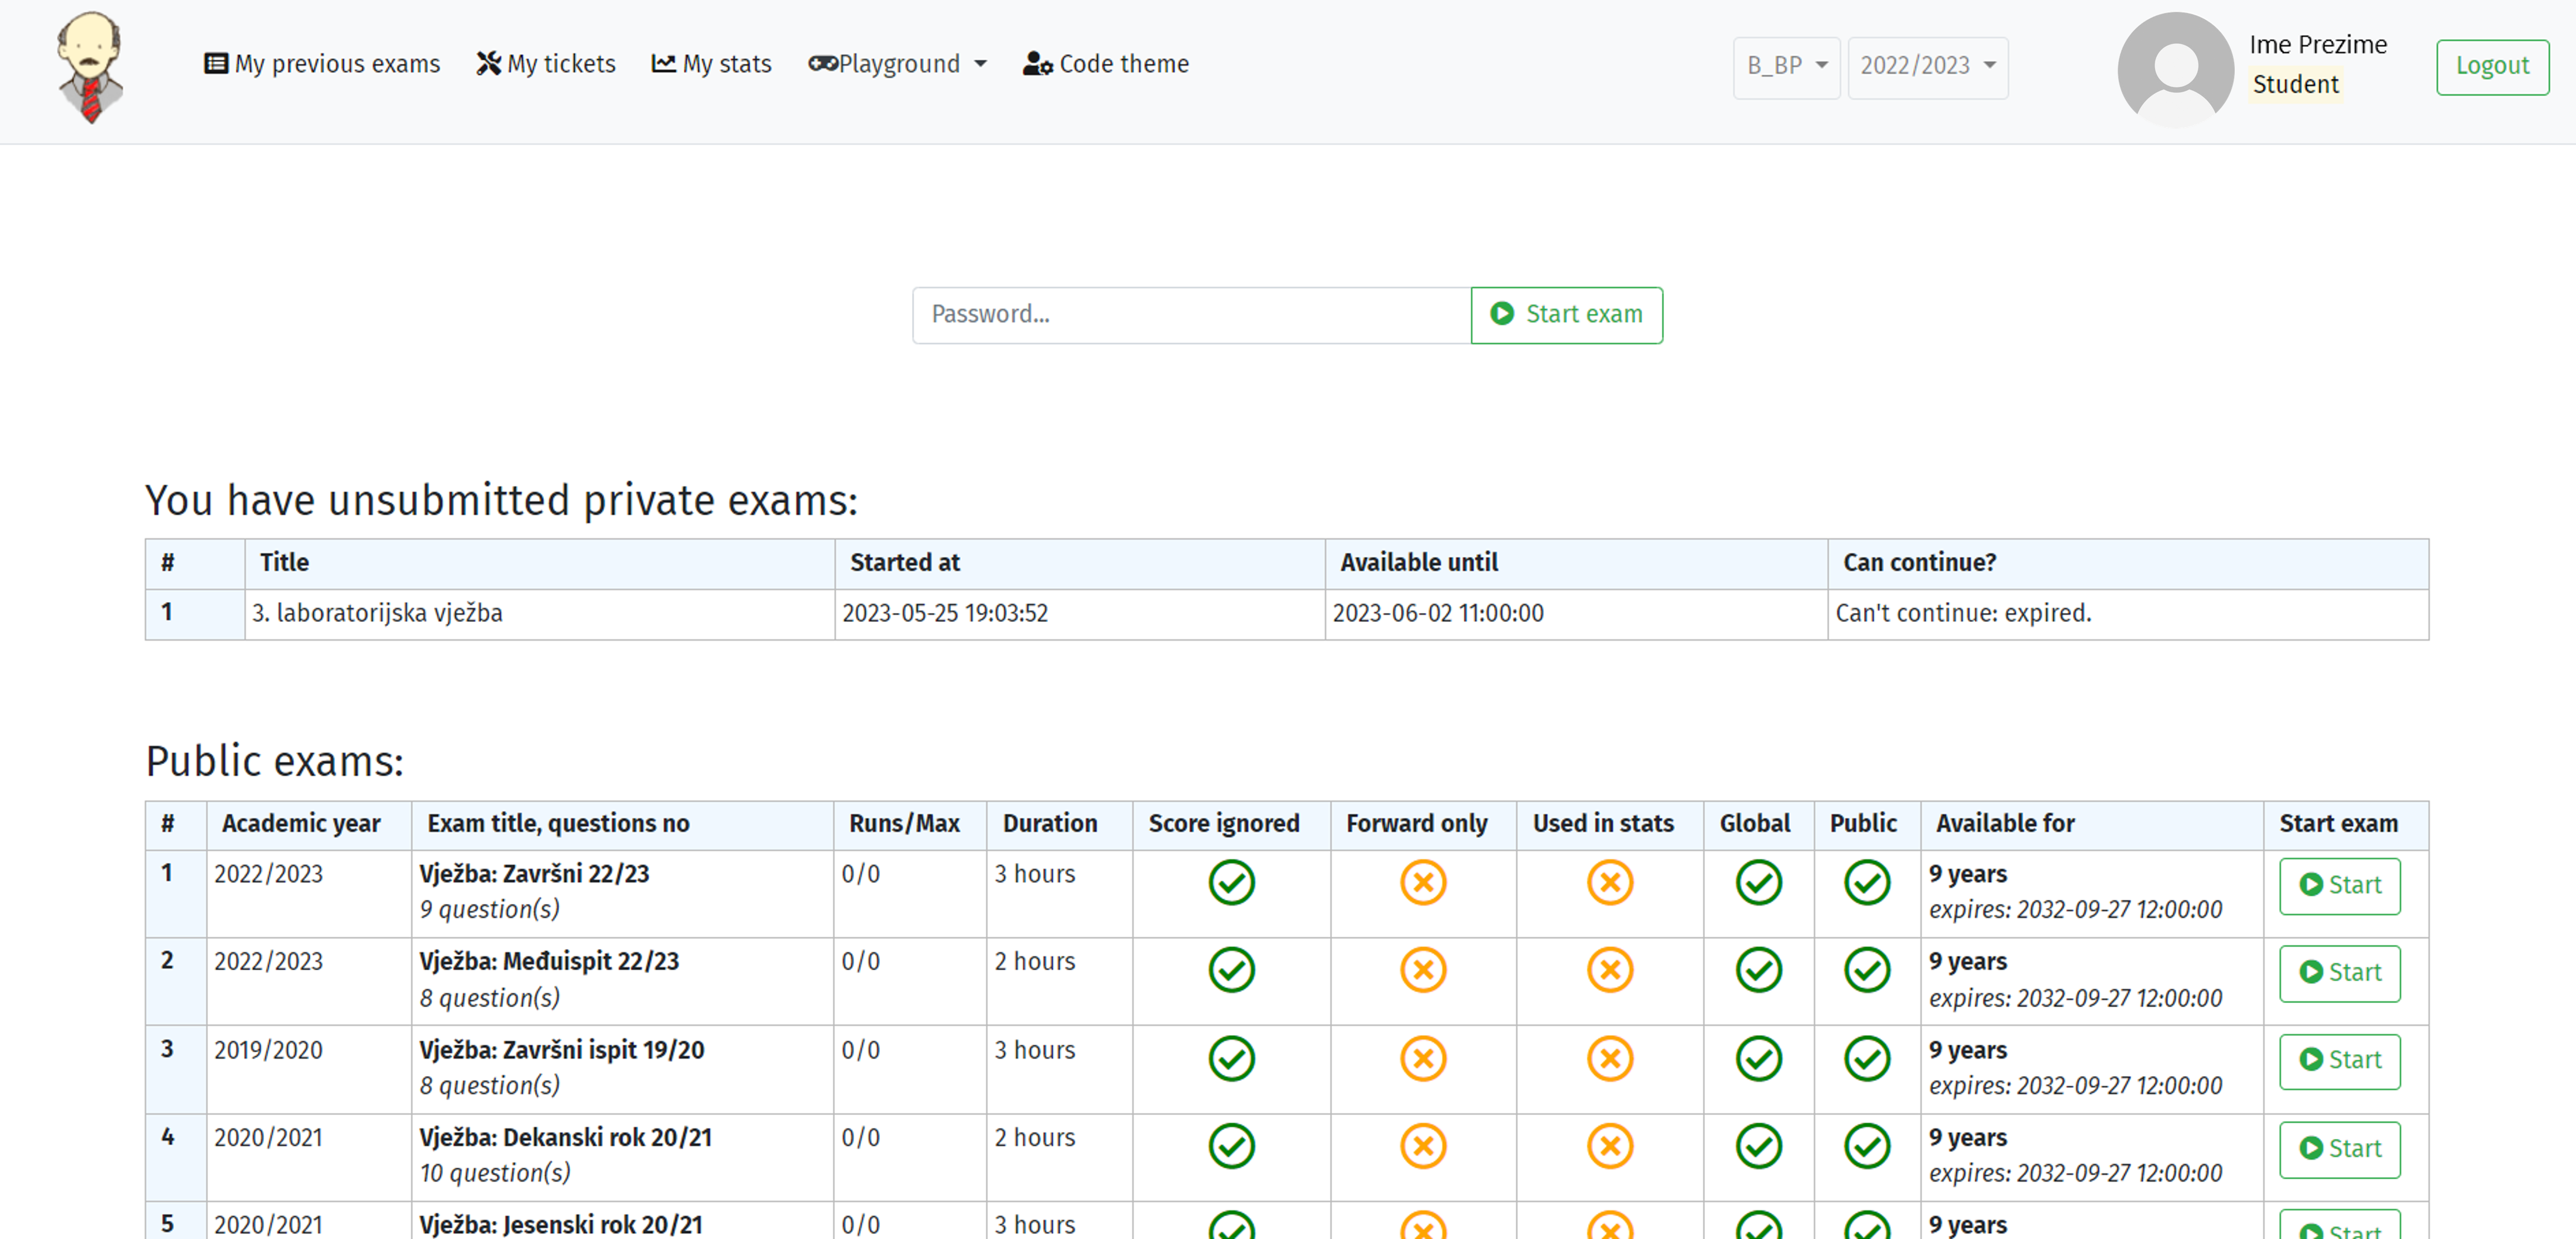
\includegraphics[scale=0.4]{slike/edgar1}
			%veličina slike u odnosu na originalnu datoteku i pozicija slike
			\centering
			\caption{Edgar: početna stranica i popis vježbi za ispite}
			\label{fig:pocstr}
		\end{figure}
				\noindent\\
		Ostale funkcionalnosti BytePita vrlo su slične Edgaru: uloge natjecatelja i studenta su slične, oni mogu učitavati i provjeravati svoj kod, pokrenuti probni ispit (slika \ref{fig:ispit}) (u BytePitu virtualno natjecanje) kao i pristupiti ispitu (odnosno natjecanju). Koncept natjecanja i ispita vrlo je sličan - korisnicima su dostupni svi ispitni zadatci istovremeno, a po završetku se ti zadatci objavljuju na stranici za vježbu. 
		Ono što u BytePitu predstavlja uloga voditelja, u Edgaru je asistent/profesor koji ima ovlasti objavljivanja tj. izrade zadataka i organizacije ispita (odabir zadataka, trajanja). U Edgaru čak postoji i stranica sa statistikom koja prikazuje uspješnost u odnosu na druge studente, postotak točno riješenih zadataka i sl.(slika  \ref{fig:stats}). BytePit ima stranicu slične namjene, ali ipak s drugačijim podatcima: na njoj natjecatelj može vidjeti tuđa rješenja i njihovu uspješnost, kao i svoj rang.	\\
		
		
			%unos slike
	
		
		\begin{figure}[H]
			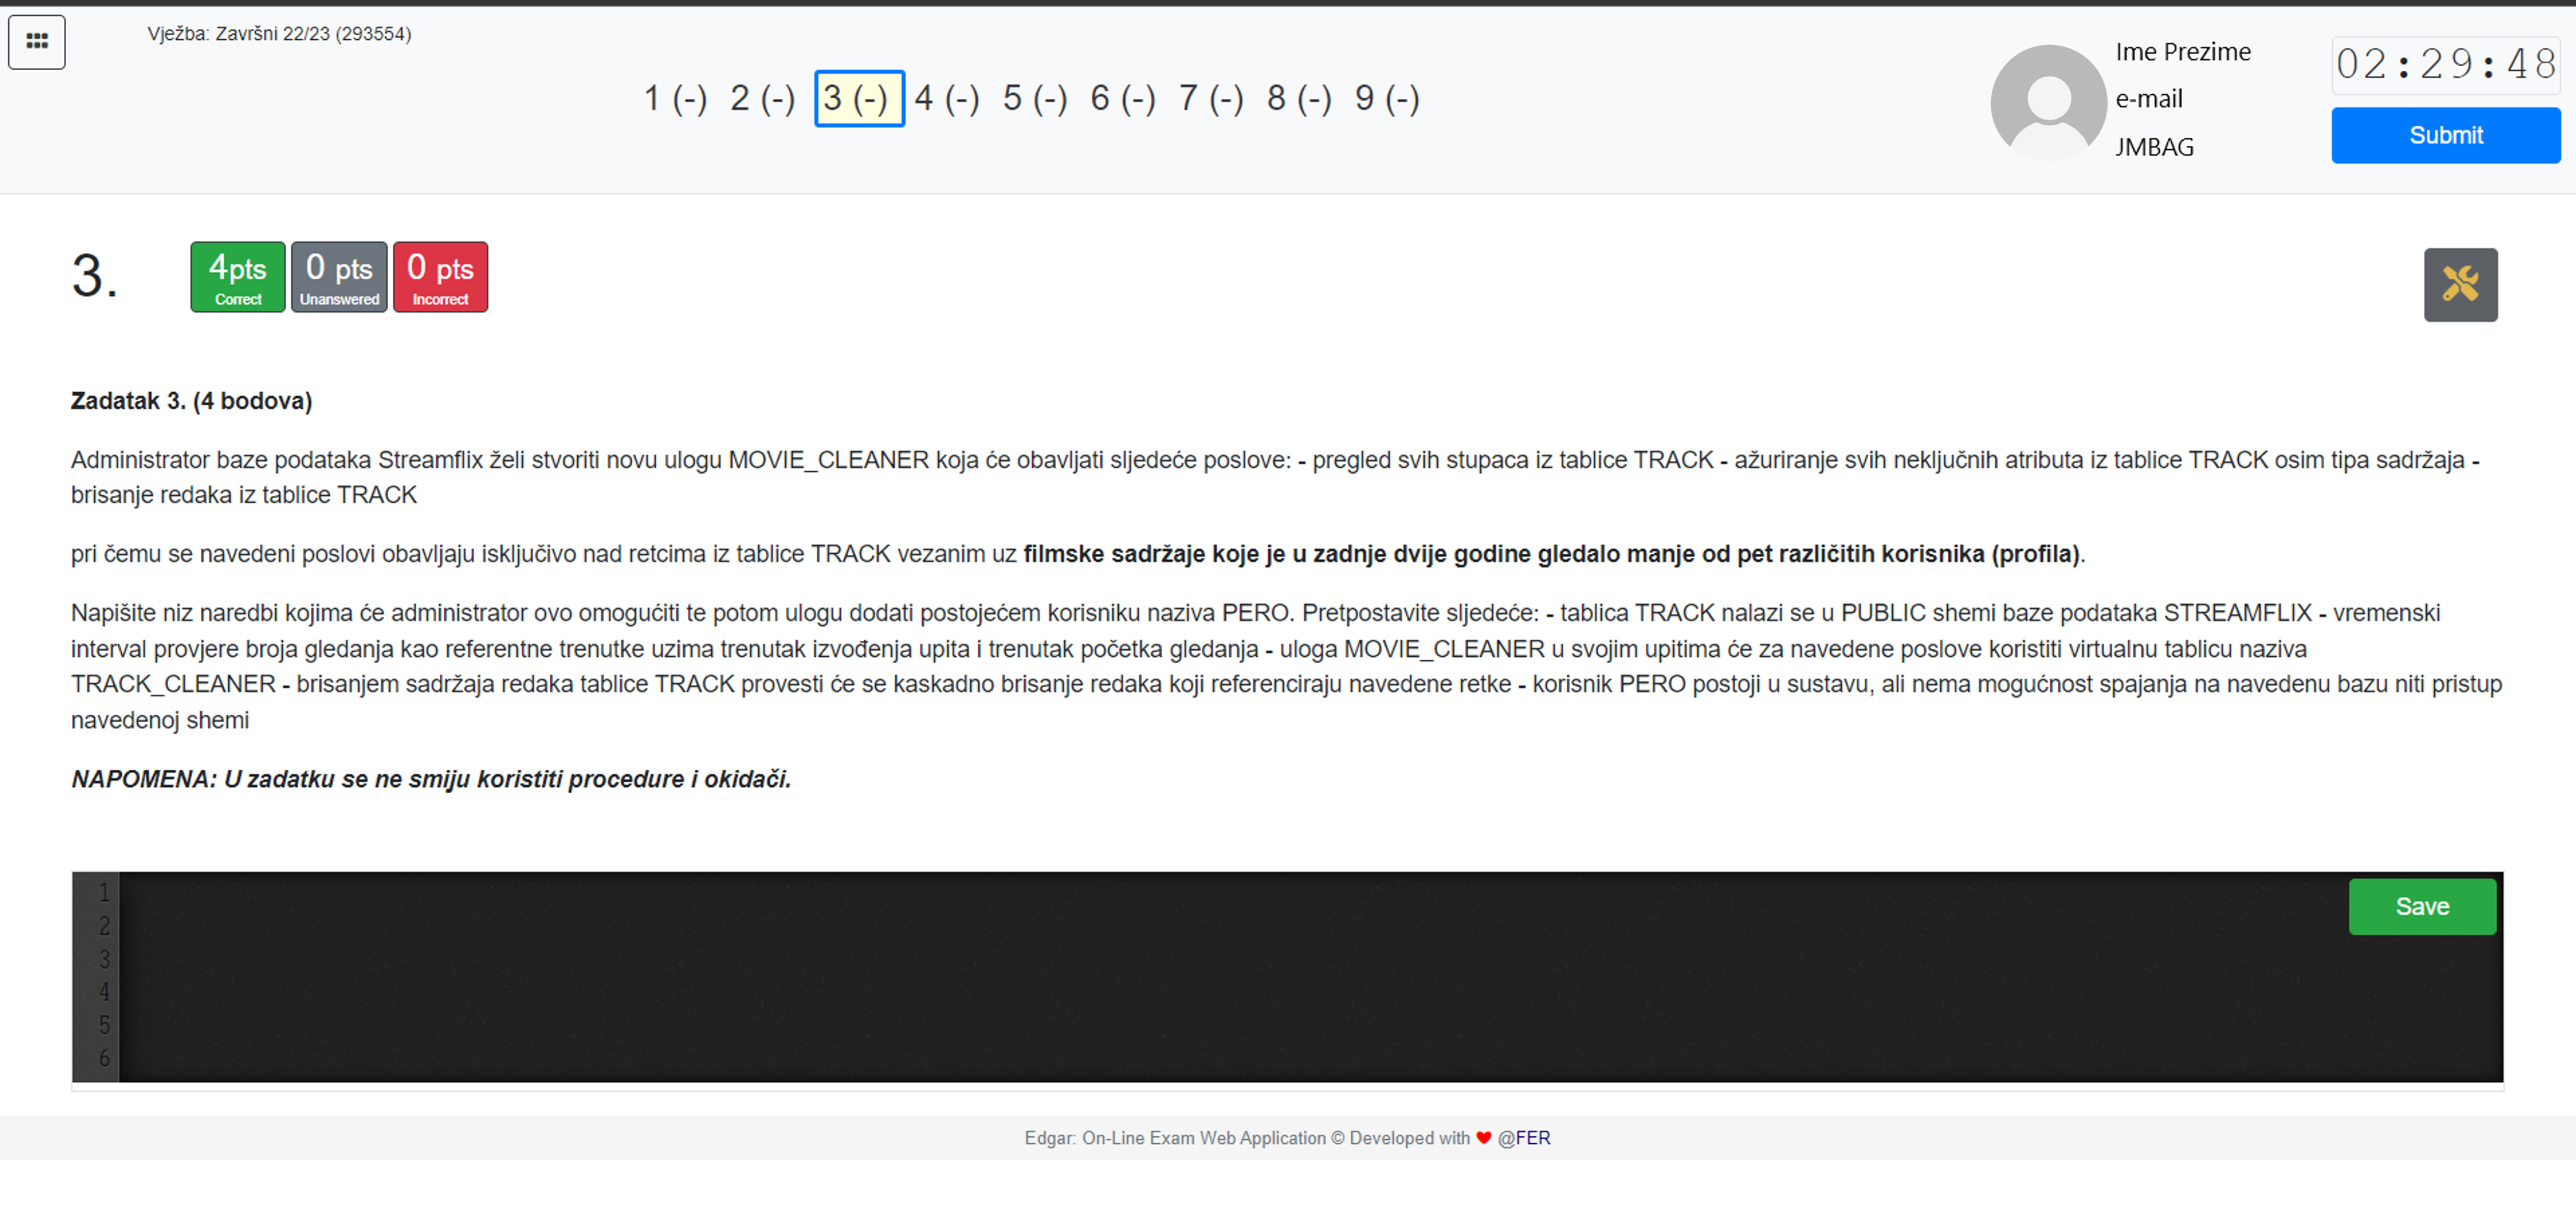
\includegraphics[scale=0.4]{slike/edgar3}
			%veličina slike u odnosu na originalnu datoteku i pozicija slike
			\centering
			\caption{Edgar: probni ispit}
			\label{fig:ispit}
		\end{figure}
		
		\begin{figure}[H]
			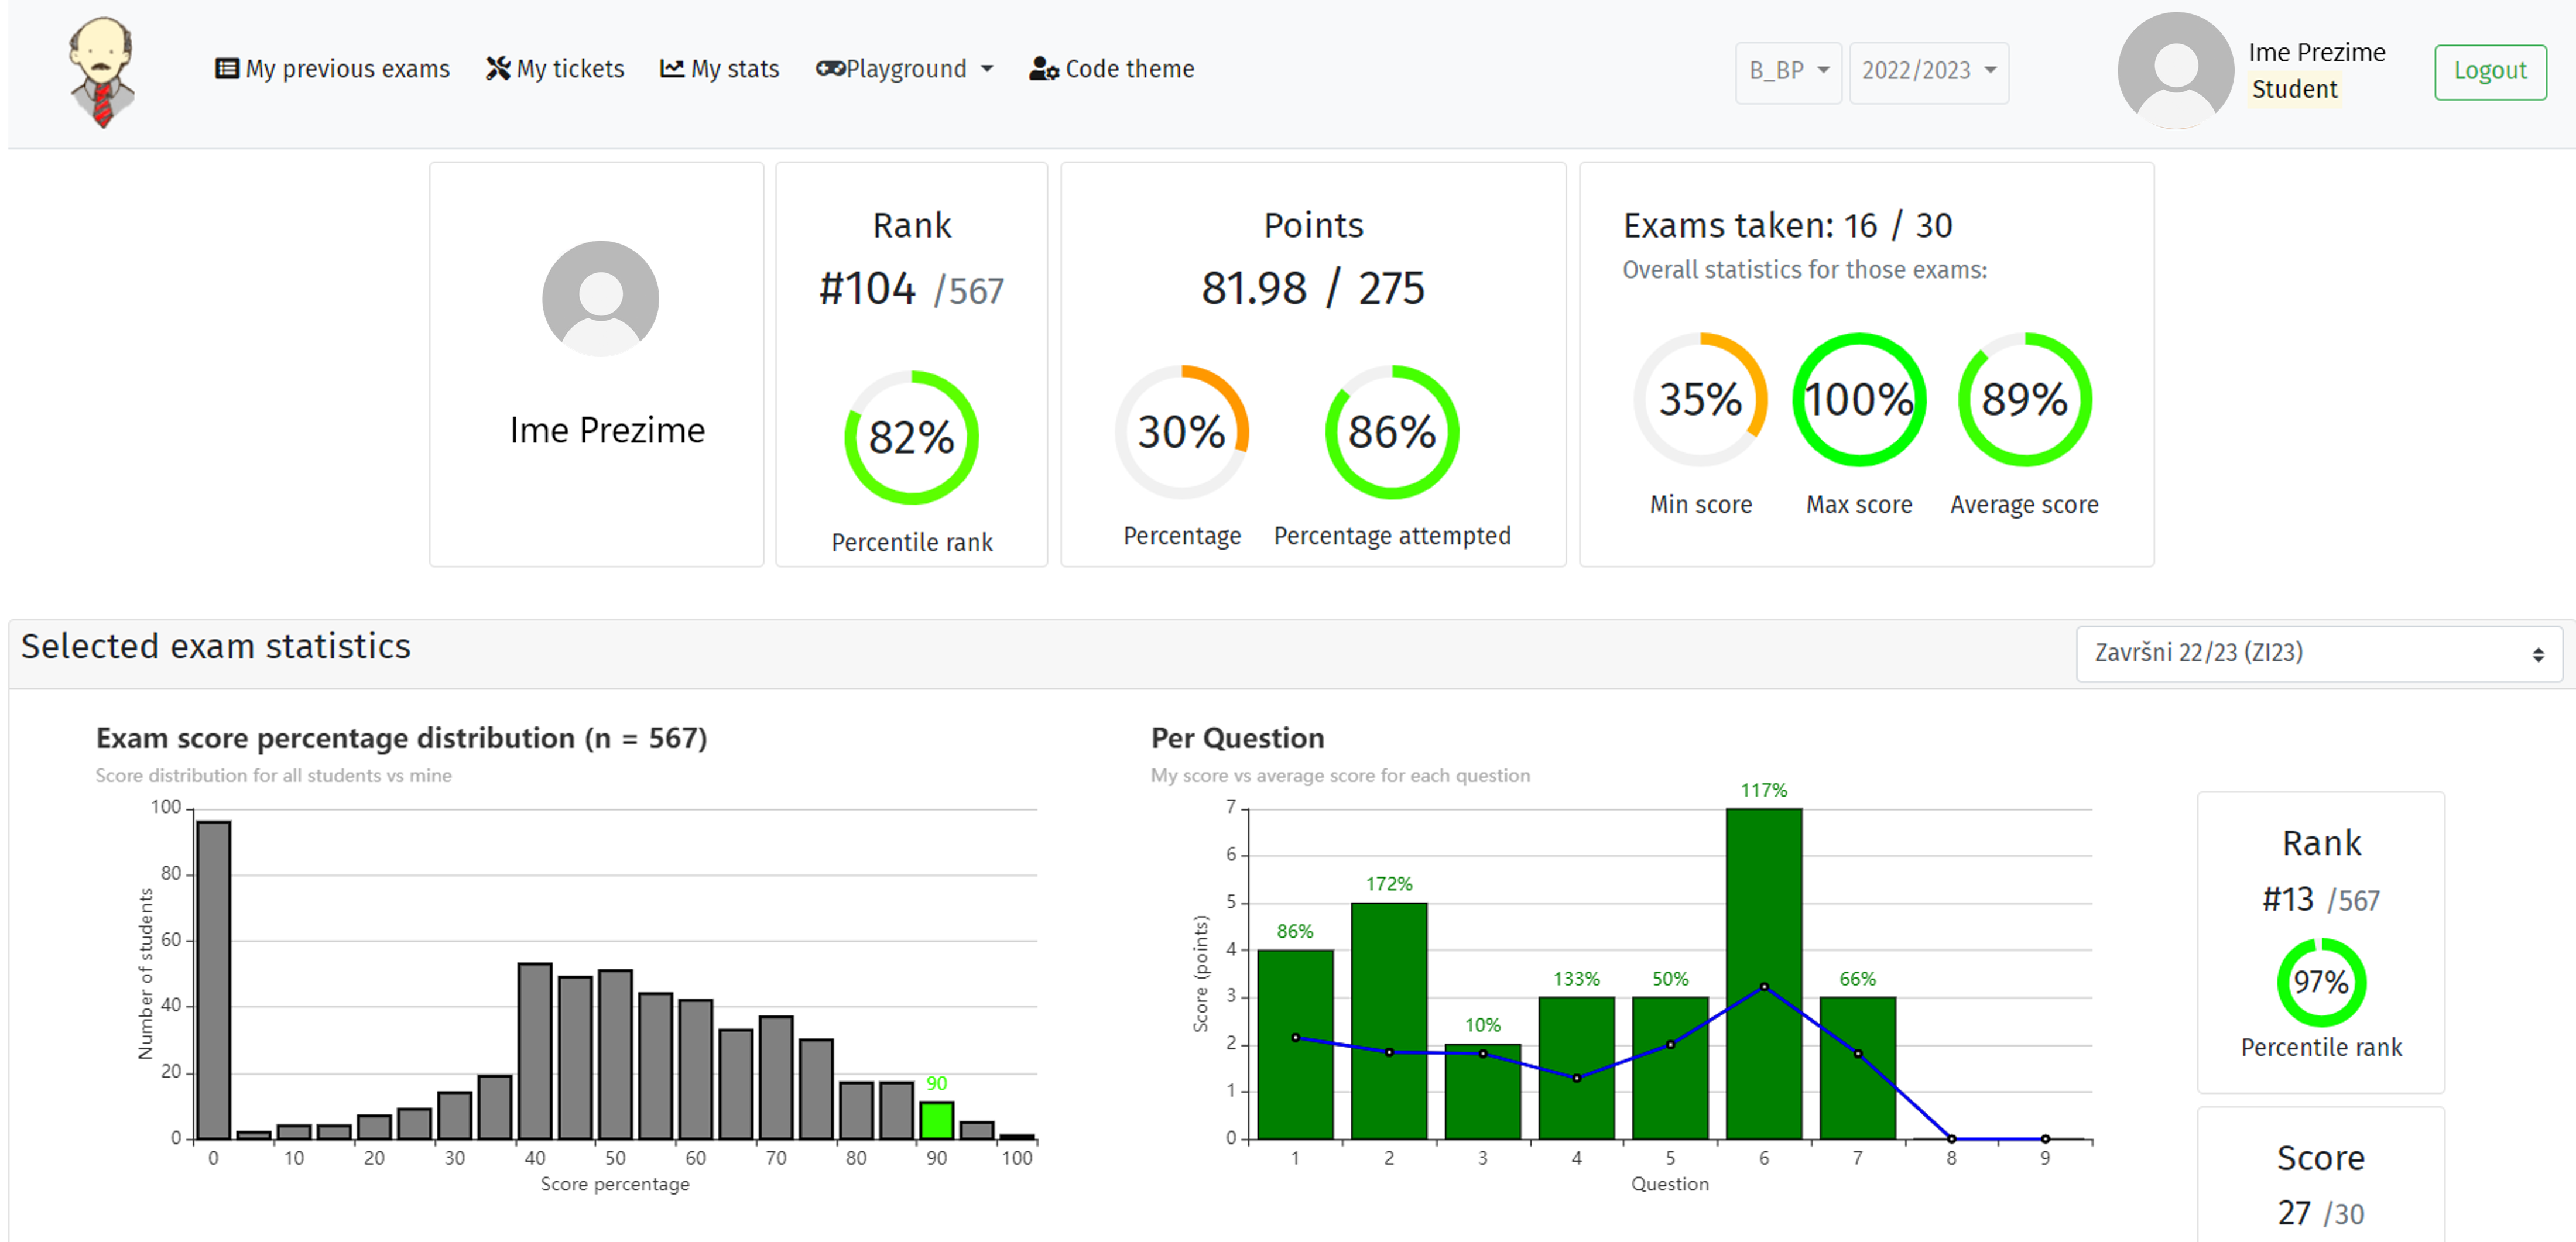
\includegraphics[scale=0.4]{slike/edgar2}
			%veličina slike u odnosu na originalnu datoteku i pozicija slike
			\centering
			\caption{Edgar: stranica sa statistikom}
			\label{fig:stats}
		\end{figure}
		
		\noindent\\
			Osim Edgara, postoji još niz aplikacija sličnih BytePitu, a jedna od njih je Codeforces, web aplikacija koja omogućuje sudjelovanje u online natjecanjima. Gotovo i da nema razlike među ovim aplikacijama: na profilima korisnika vidljiva je njihova statistika, omogućen je pristup virtualnim natjecanjima koja simuliraju prava, vidljiva je lista zadataka kao i njihovih rješenja koja su učitali korisnici (slika \ref{fig:problemi})... Ta rješenja nisu uvijek vidljiva, vidljivost ovisi o postavkama natjecanja tako je da ovisno o sudjelovanju nekim korisnicima onemogućen pregled predanih rješenja. Nasuprot tomu, u BytePitu rješenja može dohvatiti samo natjecatelj koji je i sam točno riješio zadatak. Bitna razlika u ovom je slučaju također i to što Codeforces omogućava svim korisnicima da učitaju zadatke, koji potom prolaze dodatne provjere da bi se utvrdila njihova ispravnost, dok je u BytePitu ta mogućnost otvorena samo voditeljima, i to bez dodatnih provjera nakon objave zadatka. Na profilima korisnika koji su zadatke učitali ti zadatci nisu vidljivi (u BytePitu se oni nalaze na profilima voditelja).
		Slično kao u našoj aplikaciji, nakon natjecanja moguće je na profilima korisnika vidjeti njihova rješenja i rezultate testova ali čak i bez registracije: svaki korisnik vidi rješenja svakog korisnika te nije potrebna registracija. Ono što registracija omogućuje je, dakako, sudjelovanje u natjecanjima i virtualnim natjecanjima te izvršavanje i predaja koda za riješene zadatake za vježbu (slika \ref{fig:run}) (neregistrirani korisnik može vidjeti tekst zadatka, ali ne može izvršiti kod i time provjeriti točnost rješenja). Ono što BytePit omogućuje, a Codeforces ne je mogućnost virtualnog natjecanja koje se sastoji od nasumičnih zadataka: u potonjem se nude samo replike stvarnih natjecanja koje se mogu pokrenuti. \\
		
			\begin{figure}[H]
			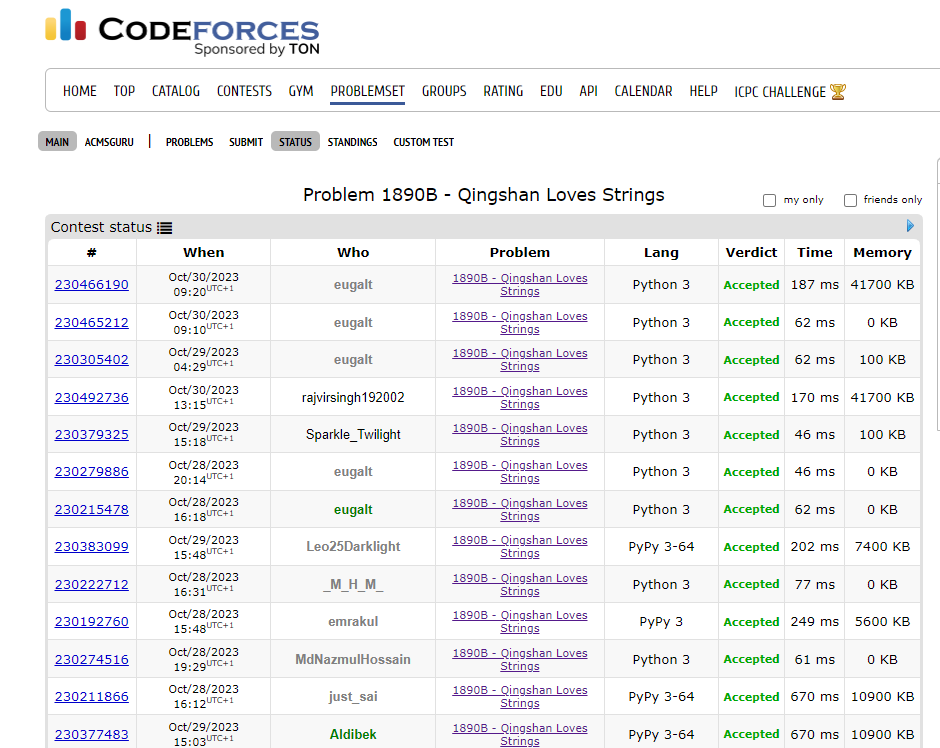
\includegraphics[scale=0.4]{slike/cf1}
			%veličina slike u odnosu na originalnu datoteku i pozicija slike
			\centering
			\caption{Codeforces: rješenja različitih korisnika}
			\label{fig:problemi}
		\end{figure}
		
		\begin{figure}[H]
			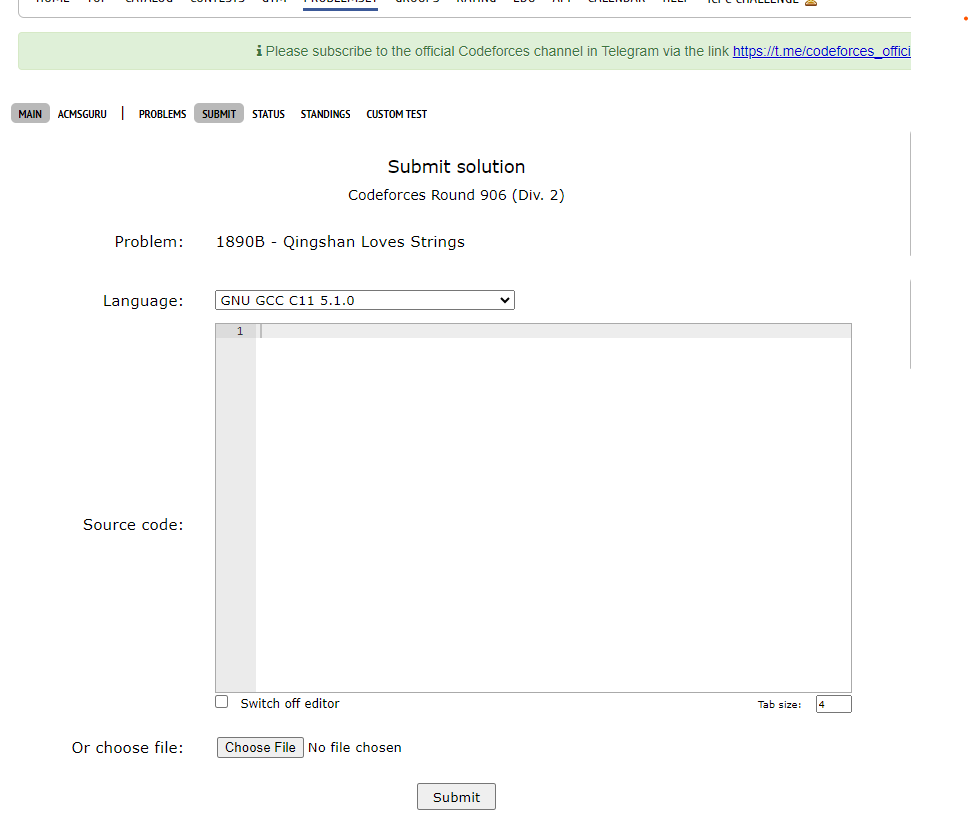
\includegraphics[scale=0.4]{slike/cf2}
			%veličina slike u odnosu na originalnu datoteku i pozicija slike
			\centering
			\caption{Codeforces: mogućnost izvršavanja koda}
			\label{fig:run}
		\end{figure}
		
		\noindent\\
		BytePit je aplikacija koja svakako može imati širu primjenu od ovdje opisane: dok je trenutna verzija aplikacije pogodna uglavnom za programerska natjecanja, s manjim preinakama ona bi se mogla koristiti u razne svrhe. Svakako bi bila dobra ideja koristiti aplikaciju kao svojevrsni test pri zapošljavanju programera odnosno za selekciju najboljih kandidata: kandidati bi dobili podatke za pristup i od njih bi se tražilo da riješe određen broj zadataka (naravno, drugačije vrste od natjecateljskih). Tako bi se lakše probralo bolje kandidate koji ulaze u uži izbor za određenu poziciju. Prilagodbom težine zadataka, BytePit bi mogao postati i platforma za vježbu i učenje programiranja. Naravno, u tom bi slučaju bilo potrebno osmisliti i kratke tečajeve programiranja, kao što to postoji na npr. Codecademy-u.
		Aplikacija bi se mogla proširiti i na način da bude slična gore predstavljenoj aplikaciji Edgar: mogla bi biti platforma za ispite iz programiranja, kako na fakultetu, tako i u osnovnim i srednjim školama.\\
		
		\eject

		
		
	